\documentclass[12pt]{standalone}
\usepackage{amsfonts, amsmath, amssymb}
\usepackage[svgnames]{xcolor}
\usepackage{tikz, pgfplots}
\usepgfplotslibrary{fillbetween}
\usetikzlibrary{shapes.geometric, calc, patterns, arrows.meta, decorations.pathmorphing}
\usepackage{mathtools}

\definecolor{gray1}{rgb}{0.5, 0.5, 0.5}
\definecolor{gray2}{rgb}{0.9, 0.9, 0.9}

\begin{document}
%
%Stern-Gerlach experiment. \par
%\begin{figure}[!h]
%	\centering
%	\begin{tikzpicture}
%	\node[draw, circle, minimum size=10pt] at (0,0) (v1) {oven};
%	\draw[very thick] (2,0.3)--(2,1.5) (2,-0.3)--(2,-1.5);
%	\draw (2,-0.9)--(v1)--(2,0.9);
%	\node[fill=blue, text=white, rectangle, minimum height=30pt, minimum width=20pt] at (3,0.9) {\textbf{S}};
%	\node[fill=red, text=white, rectangle, minimum height=30pt, minimum width=20pt] at (3,-0.9) {\textbf{N}};
%	\node at (2,-2.0) {\small collimator};
%	\draw[very thick] (5,1.5)--(5,-1.5);
%	\node[text width=2.5cm, align=center] at (5,-2.3) {\small screen \\ (expected)};
%	\draw[color=teal, thick] plot [smooth] coordinates {(5,1) (4.8,0.65) (4.2,0.28) (4.0,0) (4.2,-0.28) (4.8,-0.65) (5,-1)};
%	\draw[very thick] (7.0,1.5)--(7.0,-1.5);
%	\node[text width=2.5cm, align=center] at (7.0,-2.3) {\small screen \\ (measured)};	
%	\draw[color=teal, thick] plot [smooth] coordinates {(7,1.3) (6.8,1.0) (6.2,0.85) (6,0.65) (6.2,0.45) (6.8,0.3) (7,0) (6.8,-0.3) (6.2,-0.45) (6,-0.65) (6.2,-0.85) (6.8,-1.0) (7,-1.3)};
%	\end{tikzpicture}
%\end{figure}
%
%Stern-Gerlach measurements. \par 
%\begin{figure}[!h]
%	\centering
%	\begin{tikzpicture}
%	\tikzstyle{box} = [draw, rectangle, minimum height=1cm, minimum width=1cm];
%	
%	\node at (-1.5,0) {3.};
%	\node at (-1.5,2) {2.};
%	\node at (-1.5,4) {1.};
%	
%	\node[box] at (0,0) (s3) {$S$};
%	\node[box] at (0,2) (s2) {$S$};
%	\node[box] at (0,4) (s1) {$S$};
%	
%	\node[box] at (2,0) (az3) {$A_z$};
%	\node[box] at (2,2) (az2) {$A_z$};
%	\node[box] at (2,4) (az1) {$A_z$};
%	
%	\node[box] at (4,0) (ax3) {$A_x$};
%	\node[box] at (4,2) (ax2) {$A_x$};
%	\node[box] at (4,4) (az12) {$A_z$};
%	\node[box] at (6,0) (az32) {$A_z$};
%	
%	\draw[thick] (s3)--(az3) (s2)--(az2) (s1)--(az1);
%	\draw[thick] (2.5,4.3)--(3.5,4.3) (2.5,3.7)--(3.0,3.7) (2.5,2.3)--(3.5,2.3) (2.5,1.7)--(3.0,1.7) (2.5,0.3)--(3.5,0.3) (2.5,-0.3)--(3.0,-0.3);
%	\draw[thick] (4.5,4.3)--(5.0,4.3) (4.5,2.3)--(5.0,2.3) (4.5,1.7)--(5.0,1.7) (4.5,0.3)--(5.5,0.3) (4.5,-0.3)--(5.0,-0.3) (6.5,0.3)--(7.0,0.3) (6.5,-0.3)--(7.0,-0.3);
%	\draw[very thick, red] (3.0,3.9)--(3.0,3.5) (3.0,1.9)--(3.0,1.5) (3.0,-0.1)--(3.0,-0.5) (5.0,-0.1)--(5.0,-0.5);
%	
%	\node at (2.85,4.65) {\small $S_z^+$};
%	\node at (2.85,3.35) {\small $S_z^-$};
%	\node at (2.85,2.65) {\small $S_z^+$};
%	\node at (2.85,1.35) {\small $S_z^-$};
%	\node at (2.85,0.65) {\small $S_z^+$};
%	\node at (2.85,-0.65) {\small $S_z^-$};
%	\node at (4.85,4.65) {\small $S_z^+$};
%	\node at (4.85,2.65) {\small $S_x^+$};
%	\node at (4.85,1.35) {\small $S_x^-$};
%	\node at (4.85,0.65) {\small $S_x^+$};
%	\node at (4.85,-0.65) {\small $S_x^-$};
%	\node at (6.85,0.65) {\small $S_z^+$};
%	\node at (6.85,-0.65) {\small $S_z^-$};
%	\end{tikzpicture}
%\end{figure}
%
%Polarizers. \par
%	\begin{tikzpicture}
%\tikzstyle{box} = [draw, rectangle, minimum height=1cm, minimum width=1cm];
%
%\node at (-1.5,0) {2.};
%\node at (-1.5,2) {1.};
%
%\node[box] at (0,0) (s2) {$S$};
%\node[box] at (0,2) (s1) {$S$};
%\node[box] at (2,0) (px2) {$P_x$};
%\node[box] at (2,2) (px1) {$P_x$};
%\node[box] at (4,0) (px3) {$P_{x'}$};
%\node[box] at (4,2) (py1) {$P_y$};
%\node[box] at (6,0) (py2) {$P_y$};
%
%\node at (9.7,1) {$x$};
%\node at (9.4,1.9) {$x'$};
%\node at (8.5,2.2) {$y$};
%\node at (7.7,1.9) {$y'$};
%
%\draw[thick] (s1)--(px1)--(py1) (s2)--(px2)--(px3)--(py2)--(7,0);
%\draw[thick] (7.5,1)--(9.5,1) (8.5,0)--(8.5,2) (7.8,0.3)--(9.2,1.7) (9.2,0.3)--(7.8,1.7);
%\end{tikzpicture}

%Double-slit interference pattern. \par 
%\begin{figure}[!h]
%	\centering
%	\begin{tikzpicture}
%	\draw[thick, blue] (-3,-1)--(-3,1) (-2.67,-1)--(-2.67,1) (-2.33,-1)--(-2.33,1) (-2,-1)--(-2,1);
%	\draw[very thick, ->, blue] (-2,0)--(-1,0);
%	
%	\draw[ultra thick] (-0.7,-1.5)--(-0.7,-0.6) (-0.7,-0.4)--(-0.7,0.4) (-0.7,0.6)--(-0.7,1.5);
%	\draw[thick] (1,-1.5)--(1,1.5) (3,-1.5)--(3,1.5);
%	\node at (1,1.8) {\small individual};
%	\draw[color=cyan, thick] plot [smooth] coordinates {(1,1.5) (0.8,1.15) (0.2,0.78) (0.0,0.5) (0.2,0.22) (0.8,-0.15) (1,-0.5)};
%	\draw[color=orange, thick] plot [smooth] coordinates {(1,0.5) (0.8,0.15) (0.2,-0.22) (0.0,-0.5) (0.2,-0.78) (0.8,-1.15) (1,-1.5)};
%	\node at (3,-1.8) {\small interference};
%	\draw[color=violet, thick] plot [smooth] coordinates {(3,1.3) (2.7, 1.15) (3,1) (2.5,0.8) (3,0.6) (2.75,0.33) (2.05,0.19) (1.83,0) (2.05,-0.19) (2.75,-0.33) (3,-0.6) (2.5,-0.8) (3,-1) (2.7,-1.15) (3,-1.3)};
%	\node at (-2.5, 1.8) {\small plane wave};
%	\end{tikzpicture}
%\end{figure}

%Photoelectric effect. \par 
%\begin{tikzpicture}
%\tikzstyle{electron} = [draw, circle, minimum height=1mm, minimum width=4mm];
%
%\draw[thick] (0,0)--(10,0)--(10,2)--(0,2)--cycle;
%\draw [-{>[scale=1.5]}, line width=2, decorate, decoration={snake, amplitude=3pt, pre length=5pt, post length=5pt}, color=blue] (-0.6,6)--(1.4,4);
%\draw [-{>[scale=1.5]}, line width=2, decorate, decoration={snake, amplitude=3pt, pre length=5pt, post length=5pt}, color=blue] (-1,4.5)--(1,2.5);
%
%\node[electron] at (1,0.7) {\Huge -};
%\node[electron] at (2,1.3) {\Huge -};
%\node[electron] at (3,1) {\Huge -};
%\node[electron] at (4,1.4) {\Huge -};
%\node[electron] at (5,0.6) {\Huge -};
%\node[electron] at (5.7,1.4) (e1) {\Huge -};
%\node[electron] at (7,0.6) {\Huge -};
%\node[electron] at (7.8,1.3) {\Huge -};
%\node[electron] at (9,1.0) {\Huge -};
%\node[electron] at (7,5) (e2) {\Huge -};
%\node[electron] at (8.5,4) (e3){\Huge -};
%
%\draw [-{>[scale=1.5]}, line width=2, color=orange] (e1)--(7,3.5);
%\draw [-{>[scale=1.5]}, line width=2, color=orange] (e2)--(8.3,7.1);
%\draw [-{>[scale=1.5]}, line width=2, color=orange] (e3)--(9.8,6.1);
%
%\node at (1.9,3.3) {\large photons};
%\node at (8.5,3.3) {\large electrons};
%\end{tikzpicture}

%Quantum eraser experiment. \par 
%\begin{tikzpicture}
%\node[draw] at (-5,0) (laser) {\Large laser};
%\node[draw, thick, Navy, fill=CornflowerBlue, minimum width=5mm, minimum height=2cm] at (-0.25,0) {};
%\draw[line join=round,Cyan, fill=Cyan, rotate=22] (2.85,-0.9) arc (-15:15:3.5) arc (165:195:3.5);
%\node[draw, minimum width=1mm, minimum height=8mm, rotate=110] at (5,-1.55) {};
%\node[draw, minimum width=1mm, minimum height=8mm, rotate=22] at (4.75,-2.35) {};
%\node[draw, fill=LightSlateGray, minimum width=1mm, minimum height=2.5cm, rotate=22] at (5.1,1.9) {};
%\node[draw, minimum width=1mm, minimum height=8mm, rotate=130] at (9.85,-4.45) {};
%\node[draw, minimum width=1mm, minimum height=8mm, rotate=10] at (10.1,-3.45) {};\\
%\node[draw, minimum width=1mm, minimum height=8mm, rotate=66] at (9.5,-3.8) {};
%\node at (-0.6,2.4) {\Large double-slit screen};
%\node[text width=2cm] at (6.5,2.2) {\Large interference screen};
%\node at (0.1,-1.4) {\Large BBO};
%\node at (3.65, 0.25) {\Large lens};
%
%\draw[thick] (-0.6,-2)--(-0.6,-0.5) (-0.6,-0.37)--(-0.6,0.37) (-0.6,0.5)--(-0.6,2);
%\draw[RoyalBlue, very thick] (laser)--(-0.5,0.45);
%\draw[LimeGreen, very thick] (0,0.45)--(2.5,1.45)--(5,1.8);
%\draw[LimeGreen, very thick] (0,0.45)--(10,-3.55);
%\draw[RoyalBlue, very thick] (laser)--(-0.5,-0.45);
%\draw[DarkOrange, very thick] (0,-0.45)--(2.75,0.65)--(5,1.8);
%\draw[DarkOrange, very thick] (0,-0.45)--(9.75,-4.35);
%
%\draw[LimeGreen, very thick] (5,-1.55)--(5.5,-0.30);
%\draw[LimeGreen, very thick] (10,-3.55)--(8.3,-5.1);
%\draw[LimeGreen, very thick] (9.25,-2.02)--(9.685,-3.865);
%\draw[DarkOrange, very thick] (4.75,-2.35)--(4.25,-3.60);
%\draw[DarkOrange, very thick] (9.75,-4.35)--(9.2,-2);
%\draw[DarkOrange, very thick] (9.62,-3.83)--(8.33,-5.0);
%
%\node[draw, fill=white, minimum size=6mm, rotate=-22] at (4.25,-3.60) {\Large $B$};
%\node[draw, fill=white, minimum size=6mm, rotate=-22] at (5.5,-0.30) {\Large $A$};
%\node[draw, fill=white, minimum size=6mm, rotate=-49] at (8.2,-5.15) {\Large $D$};
%\node[draw, fill=white, minimum size=6mm, rotate=13] at (9.2,-2) {\Large $C$};
%\node[draw, circle, dashed, minimum size=4.9cm] at (9.2,-3.8) {};
%\node at (10,-1) {\Large eraser};
%
%\node[rotate=-22] at (6.55,-2.62) (splitter) {\Large splitter};
%\draw[->] (splitter)--(9.0,-3.615);
%\draw[->] (splitter)--(5.0,-2.2);
%\draw[->] (splitter)--(5.1,-1.8);
%\end{tikzpicture}
%
%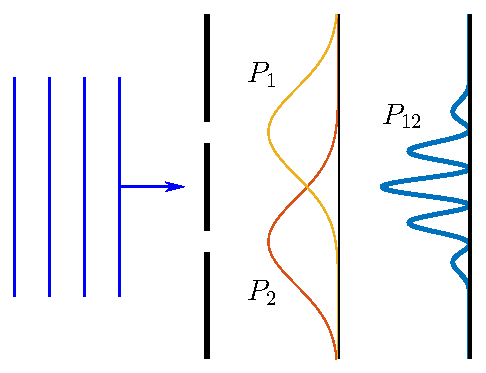
\includegraphics[width=0.6\linewidth]{double-slit}
%\put(-115,140){\large $P_1$}
%\put(-115,35) {\large $P_2$}
%\put(-50,120) {\large $P_{12}$}

%Davisson-Germer experiment. \par 
%\begin{tikzpicture}
%\node[fill=black, rectangle, minimum height=2cm, minimum width=1cm, label={0:{Nickel target}}] at (0,0) (Ni) {};
%\node[draw, rectangle, minimum height=1cm, minimum width=2cm] at (-5,0) (ebeam) {Electron beam};
%\node[text width=3cm] at (-1,3) {Diffracted \\ electron beam};
%
%\draw[->, line width=2] (ebeam)--(-2,0);
%\draw[dashed, line width=1.5] (-2,0)--(-0.5,0)--(-4,4);
%\draw[dotted, line width=1.2] (-5.4,2.5) arc (140:127:18);
%\draw[line width=1.5] (-1,0) arc (180:135:0.5);
%
%\node[draw, fill=white, rectangle, rotate=43, minimum height=7mm, minimum width=2mm, label={135:{Movable detector}}] at (-4,4) (det) {};
%\node at (-1.3,0.4) {\Large $\theta$};
%
%
%\end{tikzpicture}

%sin(x)/x. \par 
%\begin{tikzpicture}
%\begin{axis}[
%domain = 0:6.28,
%axis lines=middle,
%clip=false,
%ymin=-0.5,
%xticklabels=\empty,
%yticklabels=\empty,
%]
%\addplot+[mark=none,samples=200,unbounded coords=jump, very thick, domain=0.001:6.28] {sin(2*deg(x))/x};
%%\legend {$\frac{\sin(x)}{x}$};
%\draw[fill] (axis cs:1.57,0) circle [radius=2pt] {};
%\node at (axis cs:5.8,0.25) {\large $k_nb$};
%\node at (axis cs:-0.5,1.75) {\large $A_n$};
%\end{axis}
%\end{tikzpicture}
%
%1D potential well. \par 
%\begin{tikzpicture}
%\draw[thick] (0,3)--(0,0)--(3,0)--(3,3);
%\node at (0,-0.3) {$0$};
%\node at (1.5,-0.3) {$x$};
%\node at (3,-0.3) {$L$};
%\node at (1.5,2.6) {$V=0$};
%\node at (4.0,2.6) {$V=\infty$};
%\node at (-1.0,2.6) {$V=\infty$};
%\node [fill=red, circle, minimum size=5mm] at (1.5,0.6) (p) {};
%\draw [->, thick] (p)--(2.2,0.6);
%\draw [->, thick] (p)--(0.8,0.6);
%\fill [pattern = north east lines] (0,0) rectangle (-0.2,3);
%\fill [pattern = north east lines] (3,0) rectangle (3.2,3);
%\end{tikzpicture}
%
%particle in a box square wave function
%\begin{tikzpicture}
%\draw [thick] (0,3)--(0,0)--(3,0)--(3,3);
%\draw [thick] (1.9,0)--(1.9,1.5)--(1.1,1.5)--(1.1,0);
%\node at (0,-0.3) {$0$};
%\node at (3,-0.3) {$L$};
%\node at (1.5,2.6) {$\Psi(x,0)$};
%\node at (1.05,-0.35) {$\frac{L-b}{2}$};
%\node at (1.95,-0.35) {$\frac{L+b}{2}$};
%\node at (1.5,1.7) {$b$};
%\node at (2.1,0.7) {$A$};
%\fill [pattern = north east lines] (0,0) rectangle (-0.2,3);
%\fill [pattern = north east lines] (3,0) rectangle (3.2,3);
%\end{tikzpicture}

%Potential step. \par
%\begin{tikzpicture} [scale=0.8]
%\draw [very thick] (-4,0)--(0,0)--(0,3)--(4,3);
%\node at (1.1,1.5) {\large $V=V_0$};
%\node at (-2,-0.5) {(I)};
%\node at (2.0,-0.5) {(II)};
%\node at (-2.5, 0.4) {\large $V=0$};
%\node at (0,-0.4) {\large $x=0$};
%
%\draw [-{>[scale=1.5]}, line width=1.5, decorate, decoration={snake, amplitude=3pt, pre length=5pt, post length=5pt}, color=blue] (-5,3.8)--(-3,3.8);
%\node at (-3.5,3.1) {\large $E$};
%\end{tikzpicture}
	
%Potential barrier
%\begin{tikzpicture} [scale=0.8]
%\draw [very thick] (-4,0)--(0,0)--(0,4)--(4,4)--(4,0)--(8,0);
%\node at (1.1,2.0) {\large $V=V_0$};
%\node at (-2,-0.5) {(I)};
%\node at (2.0,-0.5) {(II)};
%\node at (6.0,-0.5) {(III)};
%\node at (-2.5, 0.4) {\large $V=0$};
%\node at (0,-0.4) {\large $x=0$};
%\node at (4,-0.4) {\large $x=L$};
%
%\draw [-{>[scale=1.5]}, line width=1.5, decorate, decoration={snake, amplitude=3pt, pre length=5pt, post length=5pt}, color=blue] (-5,3)--(-3,3);
%\node at (-3.5,2.3) {\large $E$};
%\end{tikzpicture}
%
%Tunneling cases: \par
%\begin{tikzpicture}
%		\pgfplotsset{compat=1.11}
%		\begin{axis}[
%		domain = -7:7,
%		axis line style = {draw=none},
%		tick style = {draw=none},
%		clip=false,
%		ymax = 2,
%		xticklabels = {,,},
%		yticklabels = {,,},
%		legend style = {at={(axis cs:6,1.5)}},
%		]
%		\addplot+[mark=none,samples=200,unbounded coords=jump, draw=blue, thick, domain=-7:0] {0.15*cos(deg(x)) + 0.3};
%		\addplot+[mark=none,samples=200,unbounded coords=jump, draw=orange, thick, domain=0:7] {0.45};
%		\legend {interference, transmitted particle};
%		\draw (-7,0)--(0,0)--(0,.6)--(7,.6);
%		\node at (-3.5,-0.15) {(I)};
%		\node at (3.5,-0.15) {(II)};
%		\end{axis}
%		\end{tikzpicture}

%Tunneling wave function amplitude
%\resizebox{10cm}{5cm}{
%	\begin{tikzpicture}
%		\pgfplotsset{compat=1.11}
%		\begin{axis}[
%		domain = -7:10,
%		axis line style = {draw=none},
%		tick style = {draw=none},
%		clip=false,
%		xticklabels = {,,},
%		yticklabels = {,,},
%		]
%		\addplot+[mark=none,samples=200,unbounded coords=jump, draw=blue, line width=3, domain=-7:0] {0.15*cos(deg(x+0.7)) + 0.3};
%		\addplot+[mark=none,samples=200,unbounded coords=jump, draw=orange, line width=3, domain=0:3] {0.38*exp(-0.2*x)+0.035};
%		\addplot+[mark=none,samples=200,unbounded coords=jump, draw=blue, line width=3, domain=3:10] {0.03*cos(deg(x-0.6)) + 0.267};
%		\draw [line width=1.5] (-7,0)--(0,0)--(0,.6)--(3,.6)--(3,0)--(10,0);
%		\node at (-3.5,-0.02) {(I)};
%		\end{axis}
%	\end{tikzpicture}}
%
%Oscillations T vs. E. \par
%\begin{tikzpicture}
%	\begin{axis}[
%	domain = 0:10,
%	axis lines=middle,
%	clip=false,
%	ymin=0,
%	ymax=1.001,
%	line width=1.5,
%	xlabel={\large $E$},
%	ylabel={\large $T$},
%	every axis x label/.style={
%		at={(ticklabel* cs:1.01)},
%		anchor=west,
%	},
%	every axis y label/.style={
%		at={(ticklabel* cs:1.01)},
%		anchor=south,
%	},
%	xticklabels=\empty,
%	yticklabels=\empty,
%	]
%	\addplot+[mark=none, samples=200, unbounded coords=jump, line width=2, domain=0.001:8, draw=black, dashed] {0.8};
%	\addplot+[mark=none, samples=200, unbounded coords=jump, draw=blue, line width=3, domain=0.001:8] {1/(1+pow(sin(deg(2*x))/x, 2))-0.2};
%	\node at (axis cs:-0.4,0.8) {\large 1};
%	\end{axis}
%\end{tikzpicture}
%
%Dirac comb structure. \par
%\begin{tikzpicture}
%\tikzstyle{atom} = [fill, circle, radius=2pt];
%\tikzstyle{comb} = [ultra thick, ->];
%
%%\draw [fill] (0,0) circle [radius=4pt];
%\draw [fill] (2,0) circle [radius=4pt];
%\draw [fill] (4,0) circle [radius=4pt];
%\draw [fill] (6,0) circle [radius=4pt];
%
%\draw [thick] (1,-3)--(7,-3);
%%\draw [comb] (0,-3)--(0,-1);
%\draw [comb] (2,-3)--(2,-1);
%\draw [comb] (4,-3)--(4,-1);
%\draw [comb] (6,-3)--(6,-1);
%\draw [arrows=<->, line width=1.5pt] (8,-1.5)--(8,-0.5);
%
%%\node at (0,-3.3) {\small $x=-d$};
%\node at (2,-3.3) {\small $x=-d$};
%\node at (4,-3.3) {\small $x= 0$};
%\node at (6,-3.3) {\small $x= d$};
%\node at (8,0) {Nuclei};
%\node at (8,-2) {$\delta$ Potentials};
%\end{tikzpicture}
%
%Kronig-Penney. \par
%\begin{tikzpicture}
%\pgfplotsset{compat=1.11}
%\begin{axis}[
%domain = -0.01:6.28,
%axis lines=middle,
%clip=false,
%ymin=-1.8,
%xlabel=$kd$,
%every axis x label/.style={
%	at={(ticklabel* cs:1.0)},
%	anchor=west,
%},
%xticklabels=\empty,
%yticklabels=\empty,
%legend entries={RHS, forbidden, energy bands},
%]
%\addlegendimage{line width=1.7, blue};
%\addlegendimage{pattern=north west lines, only marks, mark options={mark size=5pt, line width=0pt}};
%\addlegendimage{fill=Coral, only marks, mark options={mark size=5pt, line width=0pt}};
%
%\draw[fill, color=Coral] (0.75,1) rectangle (1.05,-1);
%\draw[fill, color=Coral] (2.1,1) rectangle (1.55,-1);
%\draw[fill, color=Coral] (3.1,1) rectangle (2.45,-1);
%\draw[fill, color=Coral] (4.2,1) rectangle (3.45,-1);
%\draw[fill, color=Coral] (4.4,1) rectangle (5.23,-1);
%
%\addplot+[line width=1.7, name path=K, mark=none,samples=200,unbounded coords=jump] {cos(deg(3*x)) + 3*sin(deg(3*x))/(2*x)};
%\addplot+[line width=1.3, name path=A, mark=none, dashed, color=SlateGray] {1};
%\addplot+[line width=1.3, name path=B, mark=none, dashed, color=SlateGray] {-1};
%
%\addplot[pattern=north west lines] fill between [of=K and A, soft clip={domain=0:0.75}];
%\addplot[pattern=north west lines] fill between [of=K and B, soft clip={domain=1.05:1.55}];
%\addplot[pattern=north west lines] fill between [of=K and A, soft clip={domain=2.1:2.45}];
%\addplot[pattern=north west lines] fill between [of=K and B, soft clip={domain=3.1:3.45}];
%\node[label={180:$1+P$}] at (axis cs:0.1,5.3) {};
%\node[label={180:$1$}] at (axis cs:0,1) {};
%\node[label={180:$-1$}] at (axis cs:0,-1) {};
%\end{axis}
%\end{tikzpicture}

%Kronig-Penney close up
%\pgfplotsset{compat=1.11}
%\begin{tikzpicture}
%\begin{axis}[
%domain = 0.5:2,
%axis lines=middle,
%clip=false,
%ymin=-1.8,
%xlabel=$kd$,
%every axis x label/.style={
%	at={(ticklabel* cs:1.0)},
%	anchor=west,
%},
%xticklabels=\empty,
%yticklabels=\empty,
%]
%\draw[fill, color=Coral] (0.75,1) rectangle (1.05,-1);
%\addplot+[line width=1.7, name path=K, mark=none,samples=200,unbounded coords=jump] {cos(deg(3*x)) + 3*sin(deg(3*x))/(2*x)};
%\addplot+[line width=1.3, name path=A, mark=none, dashed, color=SlateGray] {1};
%\addplot+[line width=1.3, name path=B, mark=none, dashed, color=SlateGray] {-1};
%\addplot[pattern=north west lines] fill between [of=K and A, soft clip={domain=0:0.75}];
%\addplot[pattern=north west lines] fill between [of=K and B, soft clip={domain=1.05:1.55}];
%\node[label={180:$1$}] at (axis cs:0.5,1) {};
%\node[label={180:$-1$}] at (axis cs:0.5,-1) {};
%\draw[fill] (axis cs:0.74,1) circle [radius=3pt] {};
%\draw[fill] (axis cs:0.87,0) circle [radius=3pt] {};
%\draw[fill] (axis cs:1.05,-1) circle [radius=3pt] {};
%\draw[fill] (axis cs:1.55,-1) circle [radius=3pt] {};
%\node at (axis cs:0.80,1.2) {$A$};
%\node at (axis cs:0.93,0.2) {$B$};
%\node at (axis cs:1.13,-0.8) {$C$};
%\node at (axis cs:1.49,-0.8) {$D$};
%\end{axis}
%\end{tikzpicture}

%Band gaps of three types of materials
%\begin{tikzpicture}
%\tikzstyle{every node} = [font=\Large]{}
%\draw[fill, color=Coral] (0,0) rectangle (3,2);
%\draw[fill, color=Coral] (4,-0.5) rectangle (7,1.5);
%\draw[fill, color=Coral] (8,-1) rectangle (11,1);
%
%\draw[fill, color=CornflowerBlue] (0,1.5) rectangle (3,3.5);
%\draw[fill, color=CornflowerBlue] (4,2) rectangle (7,4);
%\draw[fill, color=CornflowerBlue] (8,2.5) rectangle (11,4.5);
%\draw[fill, color=LightSlateGray] (0,1.5) rectangle (3,2);
%
%\draw[->, line width=3] (-0.4, -1)--(-0.4,4.5);
%
%\node at (-0.9,1.75) {$E$};
%\node at (1.5,-2) {metal};
%\node at (5.5,-2) {semiconductor};
%\node at (9.5,-2) {insulator};
%
%\node at (2,4.5) (ov) {overlap};
%\draw[very thick] (ov)--(1.5,1.75);
%\node [text width=2.5cm] at (12.5,3.5) {conduction band};
%\node [text width=2cm] at (12.22,0) {valence band};
%
%\draw[<->, line width=2] (11,2.5)--(11,1);
%\node [text width=3cm] at (12.7,1.75) {band gap};
%\end{tikzpicture}

%
%simple harmonic oscillator.
%\begin{tikzpicture}
%\node[draw, rectangle, minimum size=5mm] (m) at (3,0) {$M$};
%\draw[decoration={aspect=0.3, segment length=3mm, amplitude=3mm,coil},decorate] (0,0)--(m); 
%\fill[pattern = north east lines] (0,-1) rectangle (-0.2,1);
%\draw[thick] (0,-1)--(0,1);
%\end{tikzpicture}

%Atoms connected by springs
%\begin{tikzpicture}
%\node[fill=black, circle, minimum size=1cm] at (0,0) (a1) {};
%\node[fill=black, circle, minimum size=1cm] at (3,0) (a2) {};
%\draw[decoration={aspect=0.6, segment length=3mm, amplitude=2mm, coil}, decorate] (a1)--(a2);
%\end{tikzpicture}

%
%QHO ground state.
%\begin{tikzpicture}
%\begin{axis}[
%domain = -3:3,
%axis lines=middle,
%clip=false,
%ymin=0,
%xticklabels=\empty,
%yticklabels=\empty,
%]
%\addplot+[mark=none,samples=200, dashed, line width=2] {pow(x,2)};
%\addplot+[mark=none,samples=200, orange, line width=3] {2*exp(-pow(x,2))+1};
%\legend {parabolic potential, ground state $\psi_0$};
%\end{axis}
%\end{tikzpicture}

%Stimulated emission probability as function of omega:
%\begin{tikzpicture}
%\begin{axis}[
%domain = -10:10,
%axis lines=middle,
%clip=false,
%ymin=-0.01,
%ymax=1.2,
%xlabel=$\omega_{kl}-\omega$,
%ylabel=$P$,
%every axis x label/.style={
%	at={(ticklabel* cs:1.05)},
%	anchor=west,
%},
%every axis y label/.style={
%	at={(ticklabel* cs:1.05)},
%	anchor=south,
%},
%xticklabels=\empty,
%yticklabels=\empty,
%]
%\addplot+[mark=none,samples=200,unbounded coords=jump, line width=2] {pow(sin(deg(x))/x, 2)};
%\node[label={270:$0$}] at (axis cs:0,0) {};
%\node[label={180:$\left( \dfrac{|H'_{kl}|t}{\hbar} \right)^2$}] at (axis cs:0,1) {};
%\draw[fill] (axis cs:0,1) circle [radius=2pt] {};
%\node[label={270:$\dfrac{2\pi}{t}$}] at (axis cs:3.1416,0) {};
%\draw[fill] (axis cs:3.1416,0) circle [radius=2pt] {};
%\node[label={270:$-\dfrac{2\pi}{t}$}] at (axis cs:-3.1416,0) {};
%\draw[fill] (axis cs:-3.1416,0) circle [radius=2pt] {};
%\end{axis}
%\end{tikzpicture}

%Stimulated emission probability as function of time:
%\begin{tikzpicture}
%\begin{axis}[
%domain = 0.001:8,
%axis lines=middle,
%clip=false,
%ymin=-0.01,
%ymax=1.2,
%xlabel=$t$,
%ylabel=$P(t)$,
%every axis x label/.style={
%	at={(ticklabel* cs:1.05)},
%	anchor=west,
%},
%every axis y label/.style={
%	at={(ticklabel* cs:1.05)},
%	anchor=south,
%},
%xticklabels=\empty,
%yticklabels=\empty,
%]
%\addplot+[mark=none,samples=200,unbounded coords=jump, line width=2] {pow(sin(deg(x)), 2)};
%\addplot+[mark=none,samples=200,unbounded coords=jump, dashed, color=black] {1};
%\node[label={180:$\left( \dfrac{|H'_{kl}|}{\hbar(\omega_{kl}-\omega)} \right)^2$}] at (axis cs:0,1) {};
%\node[label={270:$\dfrac{2\pi}{|\omega_{kl}-\omega|}$}] at (axis cs:3.1416,0) {};
%\draw[fill] (axis cs:3.1416,0) circle [radius=2pt] {};
%\node[label={270:$\dfrac{4\pi}{|\omega_{kl}-\omega|}$}] at (axis cs:6.2832,0) {};
%\draw[fill] (axis cs:6.2832,0) circle [radius=2pt] {};
%%\node[label={270:$\dfrac{6\pi}{|\omega_{kl}-\omega|}$}] at (axis cs:9.4248,0) {};
%%\draw[fill] (axis cs:9.4248,0) circle [radius=2pt] {};
%\end{axis}
%\end{tikzpicture}

%Laser operation
%\begin{tikzpicture}
%\draw [-{>[scale=1.5]}, line width=1, decorate, decoration={snake, amplitude=2pt, pre length=1pt, post length=1pt}] (-0.5,0.5)--(0.5,0.5);
%\draw[fill] (0.5,0) circle [radius=2pt] {};
%\draw[->, line width=0.8] (0.5,0)--(1.4,0.9);
%\draw [-{>[scale=1.5]}, line width=1, decorate, decoration={snake, amplitude=2pt, pre length=1pt, post length=1pt}] (-0.5,0.5)--(0.5,0.5);
%\draw [-{>[scale=1.5]}, line width=1, decorate, decoration={snake, amplitude=2pt, pre length=1pt, post length=1pt}] (1.5,0.8)--(2.5,0.8);
%\draw [-{>[scale=1.5]}, line width=1, decorate, decoration={snake, amplitude=2pt, pre length=1pt, post length=1pt}] (1.5,0.2)--(2.5,0.2);
%\draw[fill] (0.5,1) circle [radius=2pt] {};
%\draw[->, line width=0.8] (0.5,1)--(1.4,0.1);
%\draw [-{>[scale=1.5]}, line width=1, decorate, decoration={snake, amplitude=2pt, pre length=1pt, post length=1pt}] (1.5,0.5)--(2.5,0.5);
%\draw[fill] (0.5,1) circle [radius=2pt] {};
%\draw[->, line width=0.8] (0.5,1)--(1.4,0.1);
%\draw (0,0)--(2,0) (0,1)--(2,1);
%\node at (-0.2,0) {$l$};
%\node at (-0.2,1) {$k$};
%\end{tikzpicture}

%% Phonon behavior
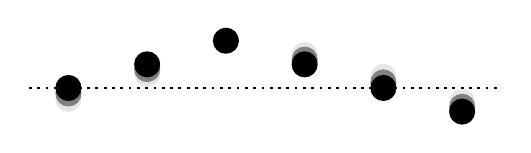
\begin{tikzpicture}
\tikzstyle{atom} = [fill, circle, minimum size=1pt];
\tikzstyle{atom2} = [fill, circle, minimum size=1pt, color=gray1];
\tikzstyle{atom3} = [fill, circle, minimum size=1pt, color=gray2];
\tikzstyle{arrow} = [<->, line width = 1pt]

\node [atom3] at (0,-0.14) {};
\node [atom2] at (0,-0.07) {};
\node [atom3] at (1,0.18) {};
\node [atom2] at (1,0.24) {};
\node [atom3] at (3,0.42) {};
\node [atom2] at (3,0.36) {};
\node [atom3] at (4,0.14) {};
\node [atom2] at (4,0.07) {};
\node [atom3] at (5,-0.18) {};
\node [atom2] at (5,-0.24) {};

\node [atom] at (0,0) {};
\node [atom] at (1,0.3) {};
\node [atom] at (2,0.6) {};
\node [atom] at (3,0.3) {};
\node [atom] at (4,0.0) {};
\node [atom] at (5,-0.3) {};

\draw [line width = 1pt, dotted] (-0.5,0)--(5.5,0);
\end{tikzpicture}
\end{document}